\documentclass{article}
\usepackage{longtable}
\usepackage{makecell}
\usepackage{float}
\usepackage{graphicx}
\usepackage{bm}
\usepackage{placeins}
\usepackage{booktabs}
\usepackage{gensymb}
\usepackage{amssymb}
\usepackage{indentfirst}
\usepackage{threeparttable} 
\usepackage{multirow}
\usepackage{aligned-overset}
\usepackage[slantfont,boldfont]{xeCJK}
\usepackage{fontspec}
\renewcommand{\arraystretch}{1.5}
\usepackage[paperwidth=20cm,paperheight=33.3cm]{geometry}
\setCJKmainfont{SimSun}
\setmainfont{SimSun}
\setsansfont{SimSun}

\title{用焦氏秤液体表面张力系数测量\\实验报告}
\author{2411545 邱凯锐}
\date{2025.5.19}

\begin{document}
\maketitle
\section{实验目的}
1.了解焦氏秤的结构、原理并学会正确使用。

2.用拉脱法测定液体的表面张力系数。

3.用最小二乘原理拟合直线

\section{实验原理}
将一表面洁净、宽度 \(L\)、丝直径为 \(D\) 的“\(\Pi\)”形细金属丝竖直地浸于水中,然后将其徐徐拉出,形成双面膜,其与水分界面接触部分的周长约为 \(2(L + D)\),因此,表面张力引起的拉力为:
\begin{equation}
f_{\alpha}=2\alpha(L + D)
\end{equation}

若将“\(\Pi\)”形丝悬挂于可测微小力的焦氏秤之上,则 \(f_{\alpha}\) 可由拉膜过程中弹簧的伸长量 \(\Delta l\) 求出。

\begin{figure}[!ht]
    \centering
    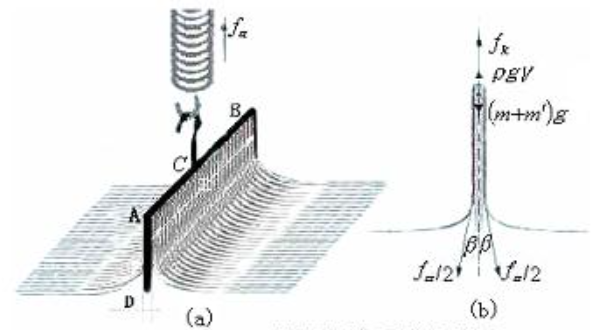
\includegraphics[width=8cm]{1.png}
    \caption{拉膜过程和受力分析示意图}
\end{figure}

实验过程中,金属丝还受到如下诸力的作用:
\begin{enumerate}
    \item 水膜自身的重力 \(m'g\) 很小可忽略;
    \item 金属丝仍处于水中的那部分体积所受到的浮力 \(\rho gV\),因金属丝框的 \(V\) 很小,故也可以忽略不计;
    \item 金属丝框受到大气压力的合力为零;
    \item “\(\Pi\)”形丝本身的重力 \(mg\),可以通过调节系统至平衡位置消除其影响。
\end{enumerate}

忽略上述作用力的影响后,弹簧的伸长就只取决于表面张力 \(f_{\alpha}\) 在垂直方向的分量。设接触角为 \(\beta\),则该分量为:\(f_{\alpha} \cos\beta\)。显然,在弹簧伸长至 \(l\) 且使液膜刚刚破裂的瞬间,该分力应与弹簧的弹性恢复力相平衡,即:
\begin{equation}
\alpha = \frac{k\Delta l}{2(L + D)\cos\beta} \label{eq:24.4}
\end{equation}

考虑到水与“\(\Pi\)”形金属丝接触角很小,\(\beta \to 0\),\(\cos\beta \to 1\);而且实际上 \(L \gg D\);所以,式(\ref{eq:24.4})可简化为:
\begin{equation}
\alpha = \frac{k\Delta l}{2L} \label{eq:24.5}
\end{equation}

其中,\(\Delta l = l - l_0\) 表示拉膜过程中弹簧的伸长量。可见,只要测得 \(k\),\(\Delta l\) 及 \(L\),即可由(\ref{eq:24.5})式求出水的表面张力系数。

\section{实验步骤}
记录实验前和实验后的环境温度$\theta_{e1}$和$\theta+{e2}$。

\subsection{测量弹簧的弹性系数$k$}
(1)组装并调节好焦氏秤,使得指示镜与指示筒不发生接触,且指示筒和指示镜的准线$E、F$和指示筒准线在指示镜中的像$E'$三线重合。

(2)用电子天平测量砝码的重量。

(3)向托盘中逐个增加砝码,每次增加完砝码后,重新将焦氏秤调节至三线重合的状态,记录砝码重量$m_i$和游标卡尺的示数$x_i$。

\subsection{拉脱法测量水的表面张力系数}
(1)用游标卡尺测量“$\Pi$”形丝的宽度$L$,测量完后用酒精灯灼烧“$\Pi$”形丝,去除其表面油污,然后将其悬挂在弹簧上。灼烧过的“$\Pi$”形丝应当用镊子夹持,避免手再次污染“$\Pi$”形丝,同时操作过程中应当小心“$\Pi$”形丝的遗失。

(2)调节焦氏秤,使得“$\Pi$”形丝恰好完全浸没在水中,且焦氏秤处于三线重合状态,记录下此时焦氏秤示数$l_0$。

(3)缓慢同时调节焦氏秤和物台的旋钮,且保持焦氏秤时刻处于三线重合的状态。将水膜缓慢拉动至刚好拉脱,记录下此时焦氏秤示数$l$。

(4)重复步骤(2)、(3),多次实验,并记录数据。

\section{实验数据以及处理}
实验室温度数据:
\begin{table}[!ht]
    \centering
    \begin{tabular}{ccc}
        \hline \hline
        $\theta_{e1}$ & $\theta_{e2}$ &  $\theta_e=(\theta_{e1}+\theta{e2})/2$\\\hline
        $298.15\ K$& $298.15\ K$& $298.15\ K$\\
        \hline \hline
    \end{tabular}
\end{table}

\subsection{测量弹簧的弹性系数$k$}
实验数据:
\begin{table}[!ht]
    \centering
    \begin{tabular}{ccccccc}
        \hline \hline
        $i$ & 1 &  2 & 3 & 4 & 5 & 6\\\hline
        $m_i(\times 10^{-3}\ kg)$ & 1.00&2.01&3.04&4.08&5.11&6.11\\
        $x_i(\times 10^{-2}\ m)$&6.75&7.66&8.59&9.5&10.46&11.37\\\hline \hline
    \end{tabular}
\end{table}

接着我们用最小二乘法得到$m-x$曲线的斜率$a_1$,进而得到弹簧的弹性系数$k$,并计算不确定度$u_k$。

斜率$a_1$与截距$a_0$:
$$
a_1=\frac{\overline{m\cdot x}-\overline{m}\cdot \overline{x}}{\overline{x^2}-\overline{x}^2}=1.1073
$$
$$
a_0=\overline{m}-a_1\cdot\overline{x}=-6.4686
$$
$$
S_{xm}=\sum_{i=1}^{6}(x_i-\overline{x})(m_i-\overline{m})=16.6173
$$
$$
S_{xx}=\sum_{i=1}^{6}{(x_i-\overline{x})^2}=15.0066
$$
$$
S_{mm}=\sum_{i=1}^{6}{(m_i-\overline{m})^2}=18.4019
$$

相关系数:
$$
r_{xm}=\frac{S_{xm}}{\sqrt{S_{xx}S_{mm}}}=0.99997
$$

不确定度:
$$
u_{m_i}=\sqrt{\frac{\sum_{i=1}^{6}{(m_i-a_0-a_1\cdot x_i)}}{6-2}}=0.0162
$$
$$
u_{a_1}=\frac{u_{m_i}}{\sqrt{S_{xx}}}=0.0042
$$    

\begin{figure}[!ht]
    \centering
    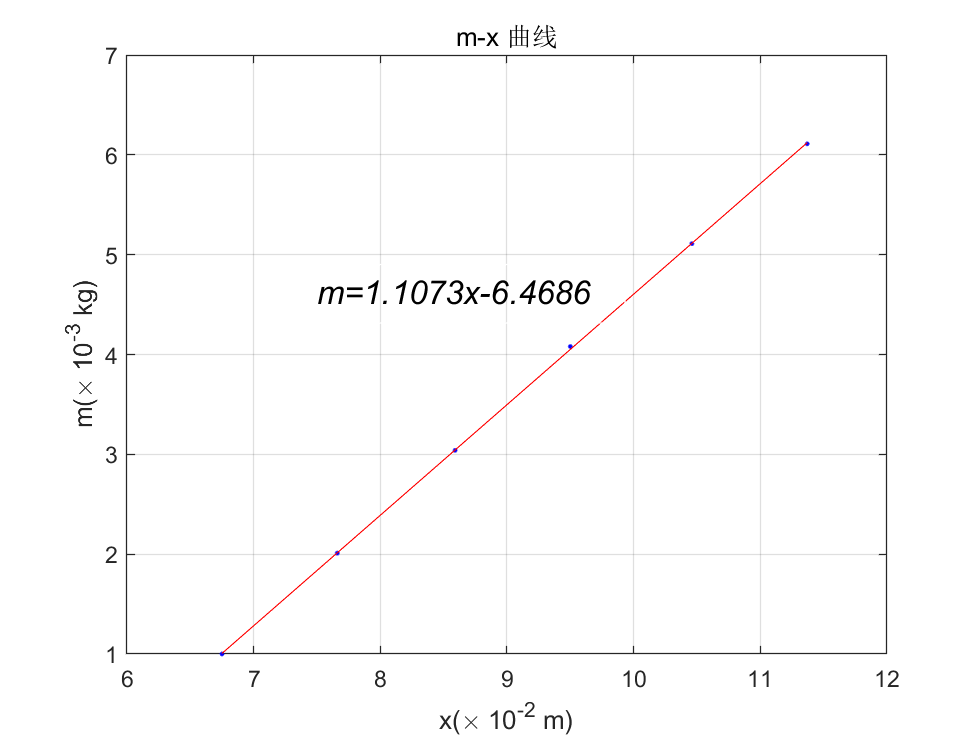
\includegraphics[width=13cm]{2.png}
\end{figure}

从而得到:
$$
    k=0.98a_1=1.0851\ N/m \quad u_k=0.98u_{a_1}=0.0041\ N/m
$$
即:$k=1.0851\pm 0.0041\ N/m$。

\subsection{拉脱法测量水的表面张力系数}
“$\Pi$”形丝宽度$L=4.1980\pm 0.0012\ cm$

实验数据:
\begin{table}[!ht]
    \centering
    \begin{tabular}{ccccc}
    \hline\hline
    $i$& 1 & 2 & 3 & 4 \\
    $l_0(\times 10^{-2}\ m)$&4.63&4.56&4.50&4.47\\
    $l(\times 10^{-2}\ m)$ &5.12&5.04&5.02&4.97\\
    $\Delta l(\times 10^{-2}\ m)$& 0.49&0.48&0.52&0.50\\
    $\alpha(N/m)$&0.0633&0.0620&0.0672&0.0646\\
    \hline\hline
    \end{tabular}
\end{table}

计算得到:$\overline{\Delta l}=0.4975\ cm$,$\overline{\alpha}=0.0643\ N/m$。

\textbf{不确定度计算}:

1.$L$的不确定度:
$$
u_L=\frac{2\times 10^{-3}\ cm}{\sqrt{3}}=1.1547\times 10^{-3}\ cm
$$

2.$\Delta l$的不确定度:
$$
S_{\Delta l_i}=\sqrt{\frac{\sum_{i=1}^{n}(\Delta l_i-\overline{\Delta l})^2}{n-1}}=0.0171
$$
$$
S_{\overline{\Delta l}}=\frac{S_{\Delta l_i}}{\sqrt{n}}=0.0085
$$
$$
u_{\Delta la}=t(0.683,3)S_{\Delta l}=0.0102\ cm
$$
$$
u_{\Delta lb}=\sqrt{2}\times\frac{1\times 10^{-2}\ cm}{\sqrt{3}}=8.1649\times 10^{-3}\ cm
$$
$$
u_{\Delta l}=\sqrt{u_{\Delta la}^2+u_{\Delta lb}^2}=0.0131\ cm
$$

3.$\alpha$不确定度:
$$
u_\alpha=\overline{\alpha}\sqrt{(\frac{u_k}{k})^2+(\frac{u_L}{L})^2+(\frac{u_{\Delta l}}{\Delta l})^2}=0.0017\ N/m
$$

得到:
$$
\alpha=\overline{\alpha}\pm u_\alpha=0.0643\pm 0.0017\ N/m
$$

\section{误差分析和思考题}
\subsection{误差分析}

由$\theta_e$计算得到:
$$
\alpha_{\theta}=B\tau^{\mu}(1+b\tau)=0.07197\ N/m
$$

相对误差:
$$
E_{\alpha}=\frac{|\alpha-\alpha_0|}{\alpha_0}\times 100\%=10.2\%
$$

误差分析:

(1)拉脱法操作精细度要求较高,难以确保拉脱时焦氏秤三线完全重合。

(2)"$\Pi$"形丝的宽度并不均匀,两边存在一定程度的弯曲。

(3)在调节旋钮的过程中,弹簧存在微小振动。

(4)测量仪器精度有限。

\subsection{思考题}

1..若“$\Pi$”形金属丝粘有油污(或用手摸过),则将会对测量结果带来什么影响?如仍采用式(3)进行计算,测量结果可能偏离真值的方向怎样?

若 “Π” 形金属丝粘有油污,会使液体对金属丝浸润性变差,削弱表面张力作用。测量时所测力偏小,如仍采用式(3)进行计算,测量结果会比真值偏小。

2.焦利氏秤为什么能测量微小力?它所能测出的最小力是多少?

焦氏秤能测量微小力是因为其弹簧劲度系数小,受微小外力时有明显伸长量,且配备精确读数装置可准确测伸长量,再依据胡克定律计算外力。其所能测出的最小力由弹簧劲度系数和读数装置精度决定,如本实验的焦氏秤(最小分度值\(0.1mm\)),最小力\(F_{min}=k\times0.1\times10^{-3}N\)($k$为弹簧劲度系数 ) 。

3.求$\alpha_{\theta}$的定值误差$E_{\alpha_{\theta}}$。

$$
E_{\alpha_{\theta}}=|\alpha-\alpha_0|=0.0077\ N/m
$$

4.试分析说明下列情况对测量结果的影响:

(1)指示镜与指示管内壁相接触;

会产生摩擦力,使弹簧伸长量测量值偏小,导致测量的外力偏小,表面张力系数测量结果偏小。

(2)确定拉膜前弹簧初始位置时AB未与水平面平齐;

会造成初始位置$l_0$测量错误,导致后续弹簧伸长量计算偏差,使表面张力系数测量结果可能偏大或偏小。

(3)拉膜时“$\Pi$”形金属丝两端4、B不在同一水平面内:

使得水膜的周长大于$2L$,导致表面张力系数的测量值大于实际值。

(4)确定平衡位置时“Ⅱ”形丝两尖端接触玻璃皿底面。

玻璃皿底面支持力使弹簧受力改变,伸长量测量偏大,导致表面张力系数测量结果偏大。


\end{document}